\section{Sombreado de Vóxeles} % (fold)
\label{sec:sombreado_de_voxeles_impl}
Para calcular la iluminación indirecta es necesario sombrear los vóxeles. Cada vóxel representa una simplificación de la radiancia saliente sobre un espacio en la escena. Llamaremos a la textura tridimensional resultante del sombreado de voxeles, \emph{textura base}. Esta información es utilizada por el algoritmo de trazado de conos para calcular la radiancia incidente sobre un fragmento.

En nuestra implementación la iluminación de los vóxeles comprende solo el componente difuso. En el proceso de voxelización se puede observar que ningún volumen está relacionado al componente especular de un material. Esto debido a dos razones: primero memoria ya que para incluir la especular durante el sombreado de vóxeles tendría que crearse otro volumen y segundo que usualmente el componente especular es un detalle fino de alta frecuencia, la voxelización siendo una simplificación de la escena podría perder detalle en especulares con lóbulos finos e incluso ocasionar errores de sombreado.

Para la iluminación de los vóxeles se utilizan técnicas de iluminación estándar en computación gráfica. La \ac{BRDF} de Lambert ya se encuentra almacenada en nuestro volumen albedo. Es necesario entonces multiplicar este valor por la atenuación normal. Para la ecuacion de renderizado ignorando la emitancia esto resulta en la siguiente ecuacion:

\begin{equation}
	\begin{split}
		L(x\to\Theta) &= \int_{\Omega_{x}}{f_{r}(x, \Psi\to\Theta)L(x\gets\Psi)\cos(N_{x}, \Psi)dw_{\Psi}}\\
		&= \int_{\Omega_{x}}{\frac{\rho}{\pi}L(x\gets\Psi)\cos(N_{x}, \Psi)dw_{\Psi}}
	\end{split}
	\label{eq:shading_voxels}
\end{equation}

El Código \ref{Shading} expone este cálculo con solo iluminación directa para los vóxeles.
\\
\begin{lstlisting}[caption={Sombreado estándar para un vóxel}, label=Shading]
vec3 BRDF(Light light, vec3 normal, vec3 albedo)
{
	// atenuación normal
	float nDotL = max(dot(normal, light.direction), 0.0f);
	// iluminación directa
	return light.diffuse * albedo * nDotL;
}
\end{lstlisting}

\begin{wrapfigure}{l}{0.3\linewidth}
	\centering
	\captionsetup{justification=centering}
	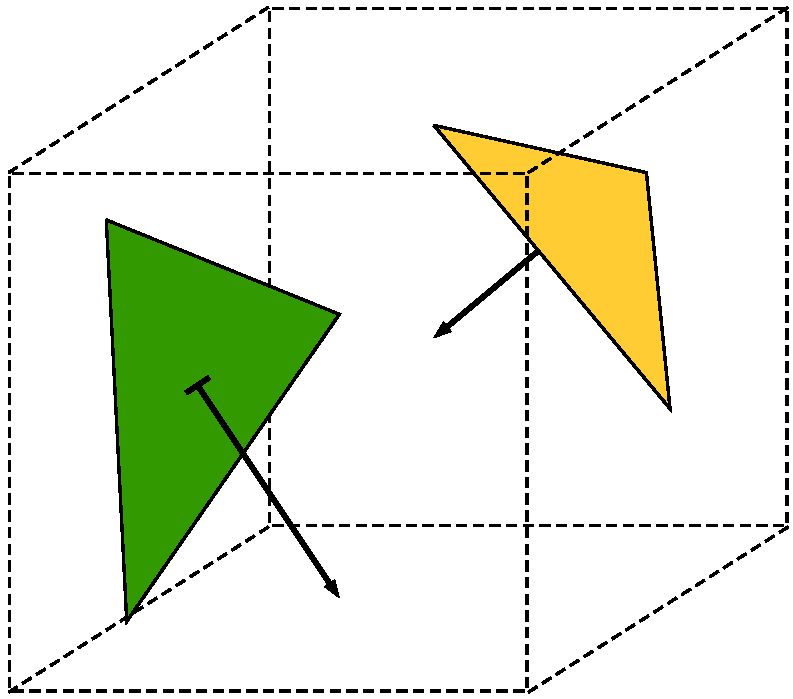
\includegraphics[width=\linewidth]{media/gimped_normals.pdf}
	\caption{Normales disparejas en un vóxel.}
	\label{fig:error_normals}
\end{wrapfigure}
Calcular el sombreado de vóxeles de esta forma es suficiente para generar resultados de buena calidad sobre el trazado de conos. Sin embargo uno de los problemas que surgen al simplificar las normales en vóxeles es que algunos vóxeles tienen normales incorrectas o desviadas. Esto sucede especialmente cuando un vóxel contiene geometría con normales muy disparejas. La Figura \ref{fig:error_normals} ilustra este fenómeno.

Para solventar esto se ideo una alternativa de sombreado sobre la atenuación normal. La idea es calcular la atenuación normal por cada cara del vóxel según la dirección de la luz $\Psi$ y luego ponderar cada atenuación normal por cara con el peso de cada eje en el vector normal. En la Figura \ref{fig:compositve_vshading} sepuede observar la composición para el sombreado final y la diferencia con Lambert tradicional. Además del método Lambert tradicional a este método lo llamamos Lambert direccional ponderado. El siguiente código expone su implementación:
\\
\begin{lstlisting}[caption={Sombreado direccional y ponderado según la normal para un vóxel}, label=Shading2]
vec3 BRDF(Light light, vec3 normal, vec3 albedo)
{
	// peso en cada eje para la normal del vóxel
    vec3 weight = normal * normal;
    // atenuación normal por cada cara del vóxel
    float rDotL = dot(vec3(1.0f, 0.0f, 0.0f), light.direction);
    float uDotL = dot(vec3(0.0f, 1.0f, 0.0f), light.direction);
    float fDotL = dot(vec3(0.0f, 0.0f, 1.0f), light.direction);
    // se encuentra la cara dominante según la normal
    rDotL = normal.x > 0.0f ? max(rDotL, 0.0f) : max(-rDotL, 0.0f);
    uDotL = normal.y > 0.0f ? max(uDotL, 0.0f) : max(-uDotL, 0.0f);
    fDotL = normal.z > 0.0f ? max(fDotL, 0.0f) : max(-fDotL, 0.0);
    // se hace un ponderado del sombreado por el peso
    nDotL = rDotL * weight.x + uDotL * weight.y + fDotL * weight.z;
    // iluminación directa
    return light.diffuse * albedo * nDotL;
}
\end{lstlisting}

\begin{figure}[H]
	\centering
	\begin{subfigure}[t]{0.2\textwidth}
		\centering
		\captionsetup{justification=centering}
		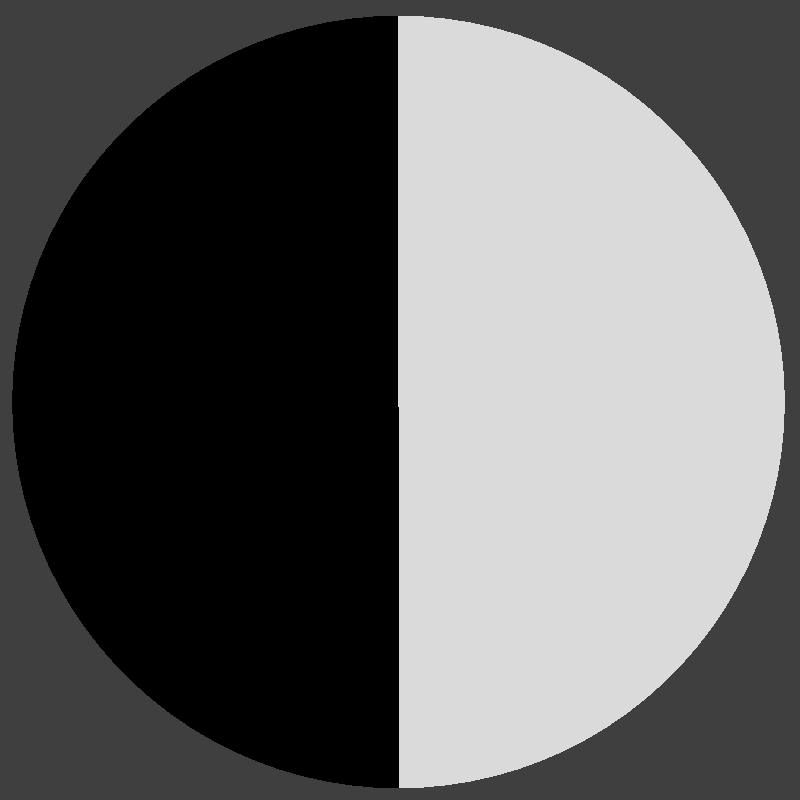
\includegraphics[width=\linewidth]{media/ndotR.png}
		\caption*{Atenuación normal, caras por eje x: \emph{rDotL}}
	\end{subfigure}%
	\begin{subfigure}[t]{0.2\textwidth}
		\centering
		\captionsetup{justification=centering}
		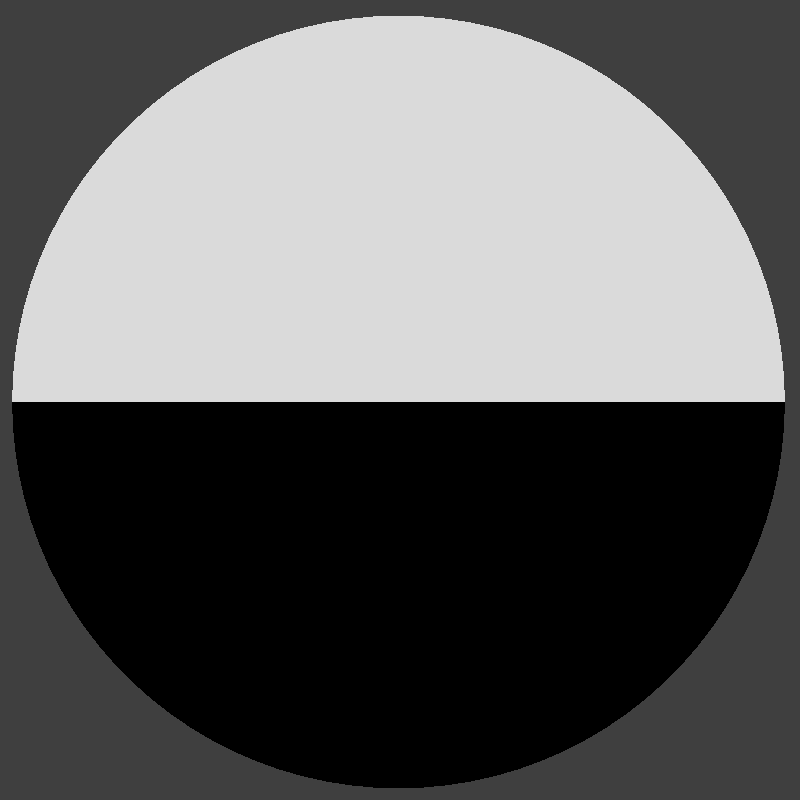
\includegraphics[width=\linewidth]{media/ndotU.png}
		\caption*{Atenuación normal, caras por eje y: \emph{uDotL}}
	\end{subfigure}%
	\begin{subfigure}[t]{0.2\textwidth}
		\centering
		\captionsetup{justification=centering}
		
\includegraphics[width=\linewidth]{media/nDotF.png}
		\caption*{Atenuación normal, caras por eje z: \emph{fDotL}}
	\end{subfigure}%
	\begin{subfigure}[t]{0.2\textwidth}
		\centering
		\captionsetup{justification=centering}
		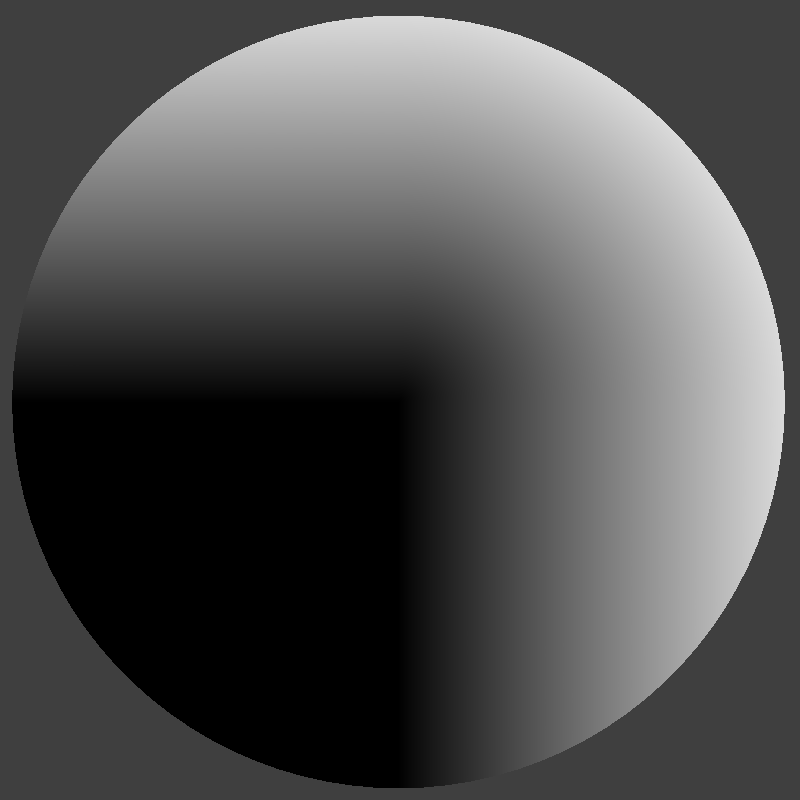
\includegraphics[width=\linewidth]{media/nDotL.png}
		\caption*{Resultado ponderado.}
	\end{subfigure}%
	\begin{subfigure}[t]{0.2\textwidth}
		\centering
		\captionsetup{justification=centering}
		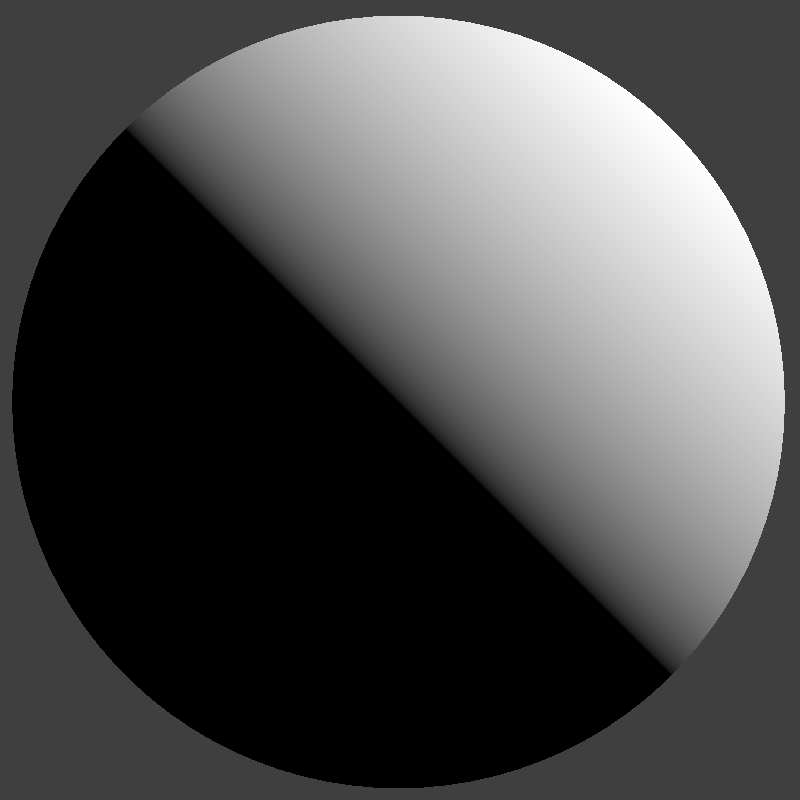
\includegraphics[width=\linewidth]{media/nDotLT.png}
		\caption*{Tradicional.}
	\end{subfigure}%
	\caption{Composición gráfica del algoritmo \ref{Shading2} para un ángulo incidente $\Theta$ y $\Psi$ de $\angle 45$ grados en BRDF Explorer \cite{brdf_explorer}.}
	\label{fig:compositve_vshading}
\end{figure}

\subsection{Mapeo y Trazado de Sombras}

Para obtener resultados coherentes también es necesario ocluir vóxeles. 

En nuestra implementación es posible utilizar mapeado de sombras solo para una luz direccional. Esta técnica es explicada en la sección \ref{subsec:shadowmapping}. La posición a proyectar $p_{v}$ es trasladada según la normal del vóxel $n_{v}$ por una distancia equivalente al tamaño medio de un vóxel en espacio de mundo $V_{wsSize}$ esto es equivalente a la siguiente ecuación: $p_{v} = p_{v} + n_{v}\cdot V_{wsSize} \cdot 0.5$. Esto se hace para evitar problemas ya explicados en la sección \ref{sub:trazado_de_sombras_sobre_el_volumen}.

Una de las ventajas de este trabajo es la capacidad de incluir muchas luces con iluminación global en escena. Por tanto es necesario alguna forma de incluir sombras para otros tipos de luces y más de una fuente de luz. Nuestra implementación realiza trazado de rayos sobre el volumen para incorporar sombras para cualquier tipo de luz dentro del área de proyección del volumen de vóxeles.

El algoritmo para detectar oclusión sobre un vóxel es simple ray tracing de un solo rayo como prueba de oclusión. Por cada fuente de luz con trazado habilitado se inicia un rayo desde la posición del vóxel a iluminar con la dirección de la luz, si este rayo colisiona con algún otro vóxel, entonces este vóxel esta ocluido.

Nuestra implementación también incluye una variación de esta técnica donde en vez de detener el rayo al colisionar, se acumulan valores a través del recorrido del rayo, estos valores decrecen según la distancia recorrida. Esto se hace para explotar el hecho de que un rayo trazado desde la posición a iluminar con la dirección de luz tendrá más colisiones al pasar por los bordes de algún objeto voxelizado visto desde esta fuente de luz (Figura \ref{fig:soft_voxel_shadow}). El propósito de esto es generar valores más claros en los bordes de la sombra para aproximar sombras suaves. El Código \ref{Shadow1} expone el trazado de rayos sobre el volumen para pruebas de oclusión:
\\
\begin{lstlisting}[caption={Trazado de rayos sobre volumen albedo para sombras sobre vóxeles}, label=Shadow1]
float TraceShadow(vec3 position, vec3 direction, float maxTracingDistance) 
{
    // tamaño de un vóxel en espacio de textura
    float voxelTexSize = 1.0f / volumeDimension;
    // se empieza el recorrido un vóxel hacia adelante para evitar auto-colisión
    float dst = voxelTexSize * 2.0f;
    vec3 samplePos = direction * dst + position;
    // visibilidad del vóxel
    float visibility = 0.0f;

    while (visibility <= 1.0f && dst <= maxTracingDistance) 
    {
        if (samplePos.x < 0.0f || samplePos.y < 0.0f || samplePos.z < 0.0f
            || samplePos.x > 1.0f || samplePos.y > 1.0f || samplePos.z > 1.0f) 
        { break; }
        
        // peso de colisión si hay algún vóxel
        float traceSample = ceil(texture(voxelAlbedo, samplePos).a) * traceShadowHit;
        // sombras duras si el valor es 1
        if(traceSample > 1.0f - EPSILON) { return 0.0f; }
        // acumulación de opacidad dividida por la distancia
        visibility += (1.0f - visibility) * traceSample / dst;
        // se marcha un vóxel hacia adelante
        dst += voxelTexSize;
        samplePos = direction * dst + position;
    }

    return 1.0f - visibility;
}
\end{lstlisting}

El valor de \emph{traceShadowHit} es definido por el usuario. Este controla el peso de cada colisión del rayo con algún vóxel. Si este valor es $1$ esto equivale a detener el rayo apenas se encuentra una colisión. La acumulación de valores se hace de manera \emph{front-to-back}, el peso de los valores acumulados disminuye con la distancia \emph{dst} recorrida del rayo.

\begin{figure}[H]
	\centering
	\begin{subfigure}[t]{0.49\textwidth}
		\centering
		\captionsetup{justification=centering}
		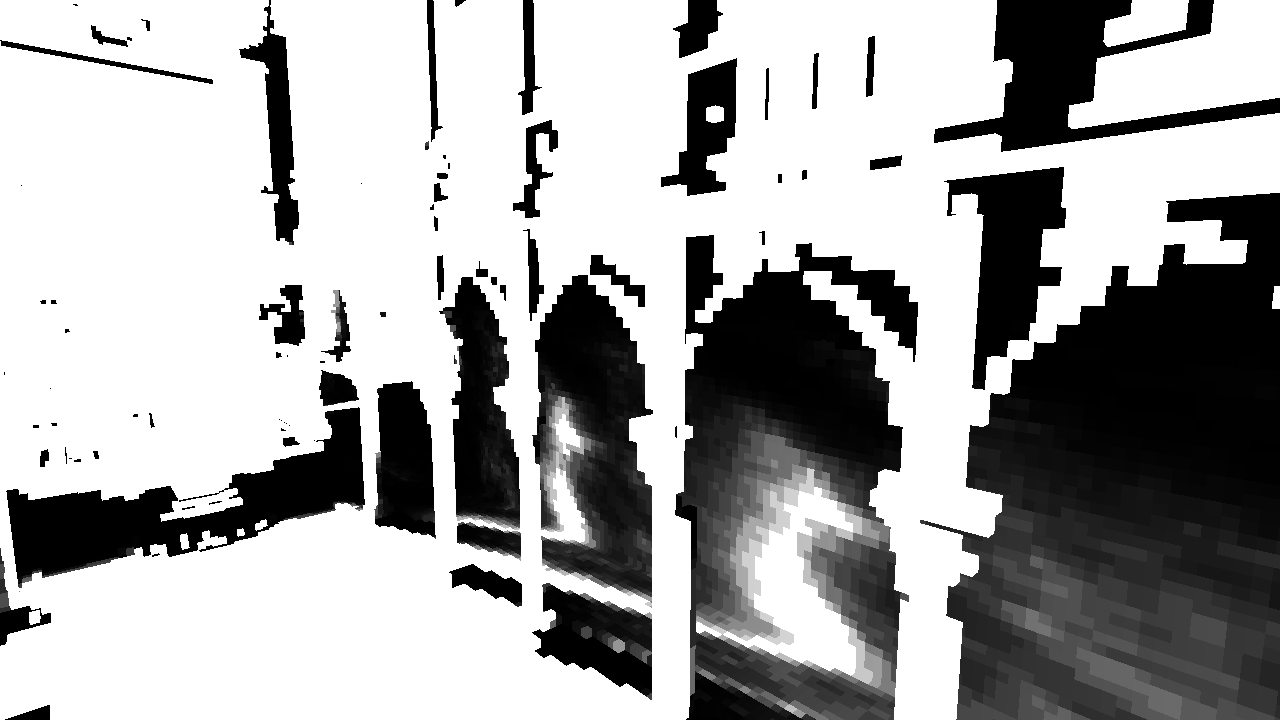
\includegraphics[width=\linewidth]{media/soft_traced.png}
		\caption*{Con trazado utilizando acumulación de colisiones.}
	\end{subfigure}%
	\hspace{0.01\textwidth}
	\begin{subfigure}[t]{0.49\textwidth}
		\centering
		\captionsetup{justification=centering}
		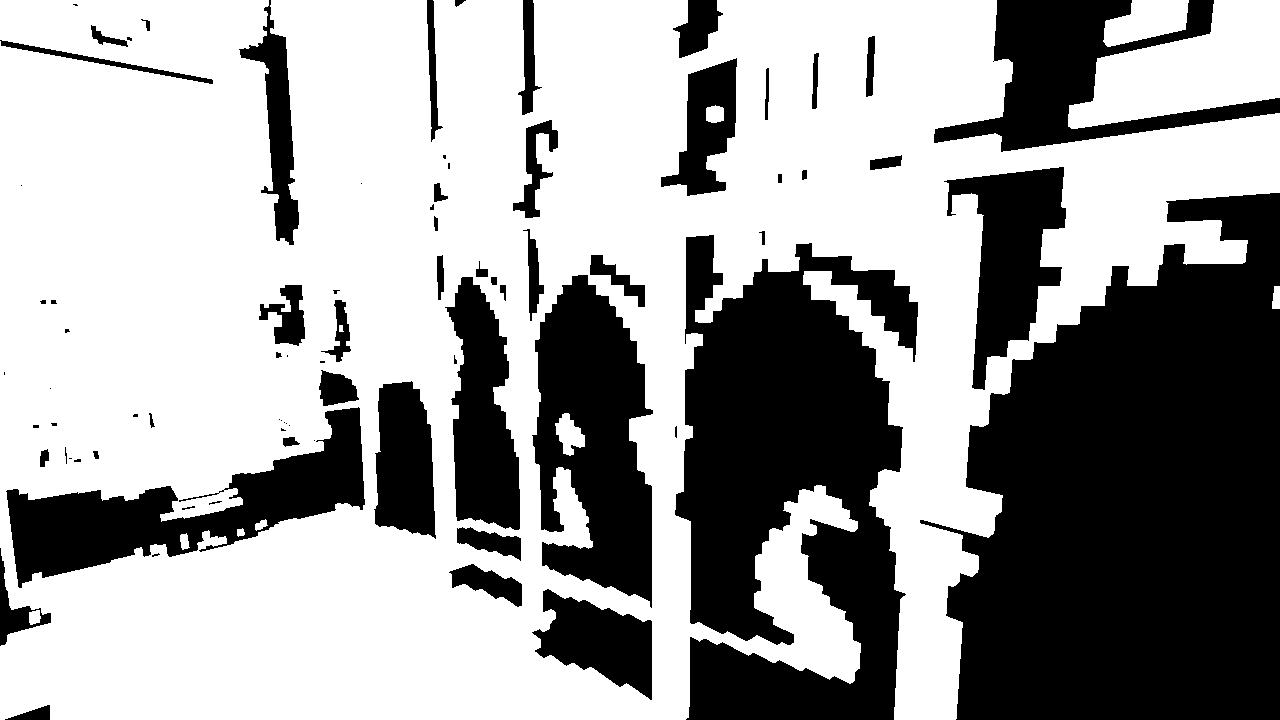
\includegraphics[width=\linewidth]{media/hard_traced.png}
		\caption*{Deteniendo el rayo de oclusión apenas colisiona.}
	\end{subfigure}%
	\caption{Valor de oclusión almacenado en el componente alfa del volumen de normales.}
	\label{fig:vshadows_hit}
\end{figure}

El valor de oclusión promedio por cada luz que traza sombras es almacenado en el componente alfa del volumen de normales, esta información puede ser utilizada para realizar mapeado de sombras con una textura tridimensional. Este componente de la textura será llamado volumen de visibilidad, en la Figura \ref{fig:vshadows_hit} se puede observar su contenido. La proyección de la posición en el volumen es mucho más sencilla que mapeo de sombras tradicional. Sin embargo la calidad es mucho más baja ya que el volumen es de baja resolución. Para proyectar la posición de un vóxel en espacio de mundo y viceversa se utilizan las dos funciones expuestas en el Código \ref{SpaceTransform}.
\\
\begin{lstlisting}[caption={Transformación de espacio entre coordenadas de textura y posiciones de mundo.}, label=SpaceTransform]
// de espacio de textura a espacio de mundo
vec3 VoxelToWorld(vec3 pos)
{
	vec3 result = pos;
	result *= voxelSize;
	return result + worldMinPoint;
}
// de espacio de mundo a espacio de textura
vec3 WorldToVoxel(vec3 position)
{
    vec3 voxelPos = position - worldMinPoint;
    return voxelPos * voxelScale;
}
\end{lstlisting}

Estas funciones son utilizadas en varias partes del algoritmo en su totalidad. \emph{VoxelToWorld} convierte una coordenada en espacio de textura a una posición en espacio de mundo, mientras que \emph{WorldToVoxel} hace lo contrario. La variable \emph{voxelSize} representa el tamaño de un vóxel dentro de la cuadrícula de vóxeles, \emph{voxelScale} representa la escala de la cuadrícula de vóxeles, \emph{worldMinPoint} es el mínimo punto de la \emph{AABB} que comprende el volumen de voxelización.

\subsection{Vóxeles Emisivos}
La forma en la que se almacenan materiales emisivos en la representación con vóxeles es muy sencilla. Al culminar el sombreado de un vóxel, al color resultante se le suma el valor de emisión obtenido del proceso de voxelización. El propósito de esto es aproximar de forma muy cruda el valor de $L_e(x\to\Theta)$, este describe la luz emitida por un punto $x$ sobre una superficie. Entonces continuando la ecuación \ref{eq:shading_voxels} ahora considerando emisión:

\begin{equation}
		L(x\to\Theta) = L_e(x\to\Theta) + \int_{\Omega_{x}}{\frac{\rho}{\pi}L(x\gets\Psi)\cos(N_{x}, \Psi)dw_{\Psi}}
\end{equation}
% section sombreado_de_vóxeles (end)

